\documentclass[11pt]{article}
\usepackage{graphicx}
\usepackage{amsmath}
\usepackage{amssymb}
\usepackage{listings}
\usepackage{color}
\usepackage{subcaption}
\usepackage[most]{tcolorbox}
\usepackage[hidelinks]{hyperref}

\definecolor{codegreen}{rgb}{0,0.6,0}
\definecolor{codegray}{rgb}{0.5,0.5,0.5}
\definecolor{codepurple}{rgb}{0.58,0,0.82}
\definecolor{backcolour}{rgb}{0.95,0.95,0.92}
\definecolor{framecolor}{rgb}{0.3,0.3,0.3}

\lstset{
    language=Python,
    basicstyle=\ttfamily\small,
    commentstyle=\color{codegreen},
    keywordstyle=\color{blue},
    numberstyle=\tiny\color{codegray},
    stringstyle=\color{codepurple},
    breakatwhitespace=false,         
    breaklines=true,                 
    captionpos=b,                    
    keepspaces=true,                 
    numbers=left,                    
    numbersep=5pt,                  
    showspaces=false,                
    showstringspaces=false,
    showtabs=false,                  
    tabsize=2,
    literate={ő}{{\H{o}}}1 {Ő}{{\H{O}}}1 {ű}{{\H{u}}}1 {Ű}{{\H{U}}}1 {é}{{\'e}}1 {É}{{\'E}}1 {–}{{--}}1
}

\newcommand{\codebox}[2][]{%
    \begin{tcolorbox}[title={Code Listing: #1}, colback=backcolour, colframe=framecolor, enhanced, fonttitle=\bfseries, breakable]
    \lstinputlisting[language=Python, nolol]{#2}
    \end{tcolorbox}
}

\title{Homework 2: Visualizing Networks}
\author{Maurice D. Hanisch}
\date{\today}

\begin{document}
\maketitle

\section*{AI Declaration}
All the first versions of the code have been written without AI. They were then debugged with AI. AI helped format this TeX file and help with the plots as well.

\section*{1. Working with real data}

\subsection*{1. a) Network Statistics and Distributions}

I analyzed the largest connected component of the researcher collaboration network ($n = 4158$). Its degree distribution and metrics are shown below:

\begin{figure}[ht]
    \centering
    \includegraphics[width=\textwidth]{figs/1a_degree_hist_and_ccdf.png}
    \caption{Degree Histogram (left) and Complementary Cumulative Distribution Function (right) for the co-authorship network.}
    \label{fig:degrees}
\end{figure}

The calculated metrics for the largest connected component are:
\begin{itemize}
    \item \textbf{Average Clustering Coefficient:} $0.5569$
    \item \textbf{Overall Clustering Coefficient:} $0.6289$
    \item \textbf{Maximal Diameter:} $17$
    \item \textbf{Average Diameter:} $6.0494$
\end{itemize}

\subsection*{1. b) Triangles and Erd\H{o}s--R\'{e}nyi Parameter}

The number of triangles $T$ in the network is $47,779$. 

To derive the expected number of triangles in an Erd\H{o}s--R\'{e}nyi graph $G(n, p)$, I consider all possible triplets of nodes. There are $\binom{n}{3}$ such triplets. For any triplet $\{u, v, w\}$ to form a triangle, the edges $(u, v), (v, w),$ and $(w, u)$ must all exist. Since edges in $G(n, p)$ occur independently with probability $p$, the probability that all three edges exist is $p \cdot p \cdot p = p^3$. 

Let $X_{i,j,k}$ be an indicator random variable that is 1 if the nodes $\{i, j, k\}$ form a triangle and 0 otherwise. The total number of triangles is $T = \sum_{1 \leq i < j < k \leq n} X_{i,j,k}$. By the linearity of expectation:
\[ \mathbb{E}[T] = \sum_{1 \leq i < j < k \leq n} \mathbb{E}[X_{i,j,k}] = \binom{n}{3} p^3 \]

Setting $\mathbb{E}[T] = T = 47,779$ and $n = 4158$, we calculate $p$:
\[ 47,779 = \binom{4158}{3} p^3 \]
\[ \implies p \approx 0.015862 \]

\subsection*{1. c) Erd\H{o}s--R\'{e}nyi Model Fit}

The Erd\H{o}s--R\'{e}nyi model does not fit this graph well. In $G(n, p)$, node degrees follow a Binomial distribution $B(n-1, p)$, which looks like a Gaussian at this scale. The actual co-authorship network is much more skewed with a heavy tail. A few authors have many papers and many connections, while the ER model stays clustered near the mean.

\begin{figure}[ht]
    \centering
    \includegraphics[width=\textwidth]{figs/1c_er_degree_distribution.png}
    \caption{Degree Histogram (left) and CCDF (right) for a generated Erd\H{o}s--R\'{e}nyi graph ($n=4158, p=0.015862$).}
    \label{fig:er_degrees}
\end{figure}

I do not need the histogram to see that ER is a poor fit. Collaboration networks cluster because a paper with $k$ authors forms a clique, creating many triangles. In a $G(n, p)$ graph, the clustering coefficient is much lower. The actual clustering coefficient here is $0.5569$. The ER model cannot replicate this inherent structure.

% \subsection*{Code Implementation: Real Data Analysis}

% The following code performs the data loading, metric calculation, and visualization for the real collaboration network.

% \codebox[Real Data Analysis]{../1_real_data_code.py}

\section*{2. Visualize your network}

For the Erdős–Rényi and SSBM models, I sampled networks with the base parameters ($n=40$ and $n=30$), but I also included examples with $n=100$ nodes (Figure \ref{fig:2a_100} and Figure \ref{fig:2b_100}). With the larger $n$, the expected structure of the graph models becomes much more apparent than with the smaller examples—specifically the uniform density of the ER model and the distinct community separation in the SSBM.

\subsection*{2. a) Erdős-Rényi Visualization}

I compared a spring layout to a circular layout for the $n=40$ ER graph. The spring layout (Figure \ref{fig:2a_spring}) provides a clear view of the connectivity, whereas the circular layout (Figure \ref{fig:2a_circular}) is less effective for recognizing local structure. For the $n=100$ version (Figure \ref{fig:2a_100}), I balanced the alpha and line width to manage the high edge density.

\begin{figure}[ht]
    \centering
    \begin{subfigure}[b]{0.45\textwidth}
        \includegraphics[width=\textwidth]{figs/2a_ER_spring.png}
        \caption{Spring Layout (n=40)}
        \label{fig:2a_spring}
    \end{subfigure}
    \hfill
    \begin{subfigure}[b]{0.45\textwidth}
        \includegraphics[width=\textwidth]{figs/2a_ER_circular_contrast.png}
        \caption{Circular Layout (n=40)}
        \label{fig:2a_circular}
    \end{subfigure}
    \caption{Erdős-Rényi visualizations showing layout comparison.}
\end{figure}

\begin{figure}[ht]
    \centering
    \includegraphics[width=0.6\textwidth]{figs/2a_ER_100.png}
    \caption{Erdős-Rényi with $n=100$ showing dense structure.}
    \label{fig:2a_100}
\end{figure}

\subsection*{2. b) SSBM Visualization}

For the SSBM, I implemented a visualization that colors nodes by their cluster ID. I also differentiated edge colors: gray for intra-cluster edges and salmon for inter-cluster edges. The spring layout (Figure \ref{fig:2b_spring}) clearly separates the communities. I also included a random layout (Figure \ref{fig:2b_random}) as a contrast; this layout is largely useless for analysis as it provides no information about the community structure.

\begin{figure}[ht]
    \centering
    \begin{subfigure}[b]{0.45\textwidth}
        \includegraphics[width=\textwidth]{figs/2b_SSBM_spring.png}
        \caption{Spring Layout (with clustering)}
        \label{fig:2b_spring}
    \end{subfigure}
    \hfill
    \begin{subfigure}[b]{0.45\textwidth}
        \includegraphics[width=\textwidth]{figs/2b_SSBM_random_contrast.png}
        \caption{Random Layout}
        \label{fig:2b_random}
    \end{subfigure}
    \caption{SSBM visualizations showing the effect of clustering.}
\end{figure}

\begin{figure}[ht]
    \centering
    \includegraphics[width=0.6\textwidth]{figs/2b_SSBM_100.png}
    \caption{SSBM ($n=100$) showing clear separation of 3 clusters.}
    \label{fig:2b_100}
\end{figure}

\subsection*{2. c) The Web}

I visualized the web graph for $n=100$ (Figure \ref{fig:2c_100_spring}) and $n=300$ (Figure \ref{fig:2c_300_spring}). I also attempted a radial/shell layout (Figure \ref{fig:2c_100_radial}), but it proved ineffective as the directed edge structure became impossible to recognize. For the $n=300$ graph, which is quite dense, I significantly reduced the alpha and edge width so that the underlying connections could still be discerned.

\begin{figure}[ht]
    \centering
    \begin{subfigure}[b]{0.45\textwidth}
        \includegraphics[width=\textwidth]{figs/2c_Web100_spring.png}
        \caption{n=100 (Spring)}
        \label{fig:2c_100_spring}
    \end{subfigure}
    \hfill
    \begin{subfigure}[b]{0.45\textwidth}
        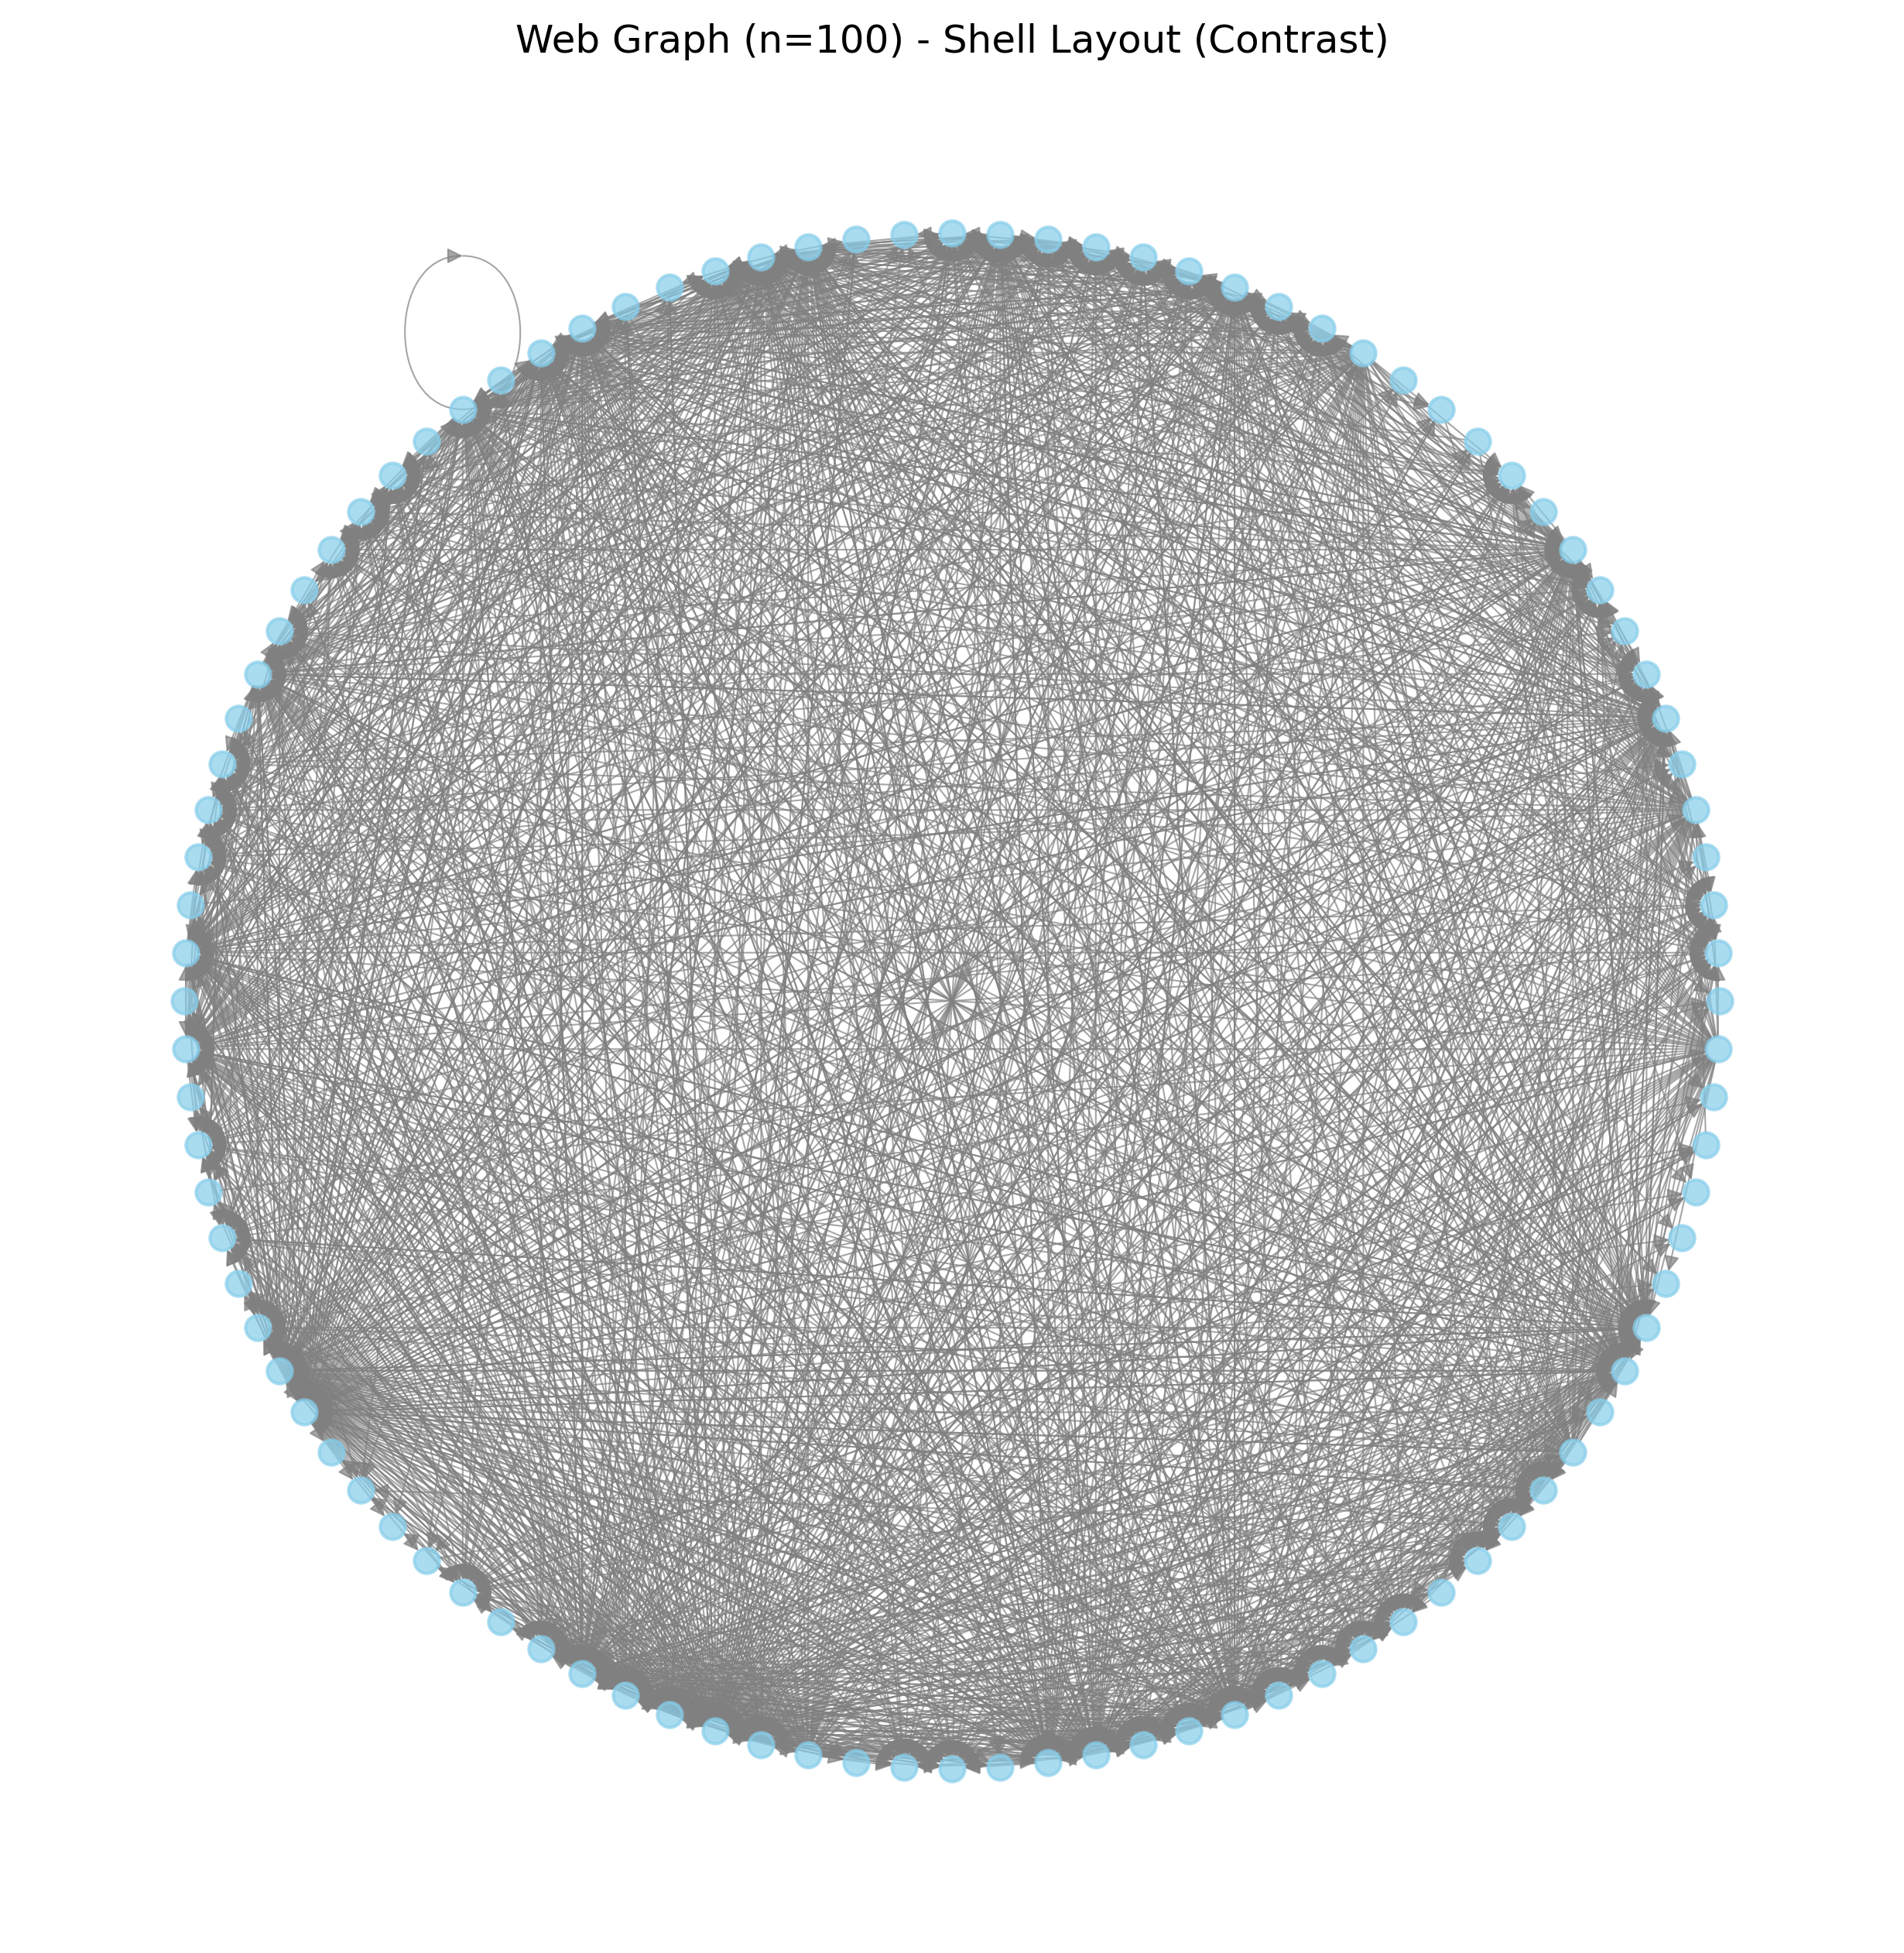
\includegraphics[width=\textwidth]{figs/2c_Web100_radial_contrast.png}
        \caption{n=100 (Radial/Shell)}
        \label{fig:2c_100_radial}
    \end{subfigure}
    \caption{Web graph visualizations.}
\end{figure}

\begin{figure}[ht]
    \centering
    \includegraphics[width=0.6\textwidth]{figs/2c_Web300_spring.png}
    \caption{Web graph with $n=300$ using balanced alpha and width.}
    \label{fig:2c_300_spring}
\end{figure}

\subsection*{Code Implementation}

The following code generates and visualizes these networks. It is imported directly from the notebook.

\codebox[Visualization Generation]{../2_visualize_code.py}


\section*{3. The Navigation Paradox}

\subsection*{3. a) \& b) Graph Generation and Distance}

I generated a connected Watts-Strogatz graph with $n=1000$, $k=10$, and $p=0.1$. I implemented the ring distance function $d_{ring}(u, v) = \min(|u-v|, n - |u-v|)$.

\subsection*{3. c) Path Length Comparison}

I compared the true shortest path length with the path length found by a greedy search for 100 random pairs.

\begin{itemize}
    \item \textbf{Average Shortest Path Length:} 4.48
    \item \textbf{Average Greedy Path Length:} 12.99
\end{itemize}

The greedy search performs significantly worse than the optimal path, and in some cases, it can get stuck or take very long routes.

\subsection*{3. d) Why Greedy Search Fails}

The greedy agent fails to utilize the random shortcuts effectively because it relies solely on local geometric information (the 1D ring distance) to make routing decisions.

In the Watts-Strogatz model, the "shortcuts" are added (or rewired) uniformly at random; they are not correlated with the underlying geometry of the ring. A greedy agent will only take a shortcut if it lands strictly closer to the target in terms of ring distance. This approach misses opportunities to take shortcuts that might initially appear to move away from or stay roughly equidistant to the target on the ring, but actually connect to a "highway" leading very close to the destination. 

\subsection*{Code Implementation: Navigation}

\codebox[Navigation Simulation]{../3_navigation.py}

\end{document}
